
% This LaTeX was auto-generated from an M-file by MATLAB.
% To make changes, update the M-file and republish this document.

\documentclass{article}
\usepackage{graphicx}
\usepackage{color}
\usepackage{listings}
\usepackage[framed]{mcode}
\usepackage{fullpage}
\usepackage{amsmath}
\usepackage[utf8x]{inputenc}
\usepackage{import}
\usepackage{setspace}
\usepackage{hyperref}
\definecolor{lightgray}{gray}{0.5}
\setlength{\parindent}{0pt}

\begin{document}

    
    \begin{lstlisting}
clc; close all; clear;

% <latex>
% \title{BE 521: Homework 3 Questions\\{\normalsize Feature extraction} \\{\normalsize Spring 2021}}
% \author{68 points}
% \date{Due: Tuesday, 2/16/2021 10pm}
% \maketitle
% \textbf{Objective:} Extract features from data and build a simple detector
% </latex>
\end{lstlisting}

\begin{center}
\author{Shubhankar Patankar \\
  \normalsize Collaborators: Peter Galer \\}
\end{center}


\section{Features and Simulations (39 pts)} As you learned
in class, features are the backbone of almost all detection
strategies, from seizures in EEG to faces in images. Features are
usually defined in journal articles as an equation or set of
equations, and the task for the reader---if she wants to use that
feature---is to implement that feature in code. In this section, you
will explore and implement some features commonly used in EEG
analysis and test them on simulated time-series data.
\begin{enumerate}
 \item Consider the following toy signal: 7 seconds of a 2 Hz sine
 wave with a quarter period phase-shift, sampled at 100 Hz
  \begin{enumerate}
   \item Plot the signal. (2 pts)

\begin{lstlisting}
cd('/Users/sppatankar/Developer/BE-521')
addpath(genpath('Homework_3'));

duration = 7; % s
sampling_rate = 100; % Hz
dt = 1/sampling_rate;
time = 0:dt:7-dt;
signal_frequency = 2; % Hz
period = 1/signal_frequency;
toy_signal = sin((2 * pi * signal_frequency * (time + (0.25 * period))));

figure;
plot(time, toy_signal, 'LineWidth', 1, 'Color', [0, 0, 0])
xlabel('Time (s)', 'FontSize', 15);
ylabel('Signal', 'FontSize', 15);
title('Toy Signal', 'FontSize', 15);
\end{lstlisting}


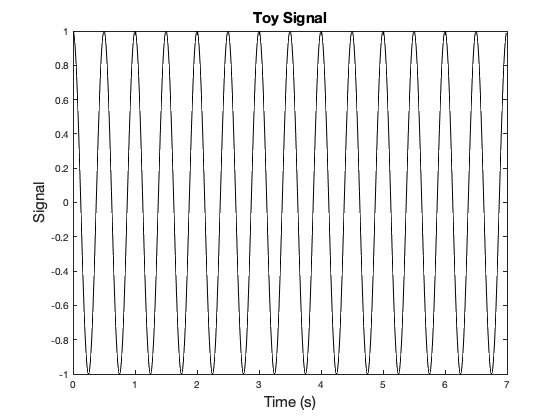
\includegraphics [width=5in]{spatank_hw3_01.png}

\item Using the Matlab functions for the difference, sum, and
  absolute value of the elements in a vector (look them up if you
  don't know them), create an anonymous function for the
   line-length feature
	$ LL(\mathbf{x}) = \sum_{i=2}^{n} |x_i - x_{i-1}| $ in one line of
	Matlab code that uses no loops (i.e., the outputs of one function
	will be the inputs of another). Your function should look
	something like \begin{lstlisting}
	  LLFn = @(x) XXXXXX;
	\end{lstlisting}
	where \texttt{XXXXX} represents some use of the aformentioned functions and the input signal \texttt{x}. (4 pts)
   \item What is the line length of this signal? (2 pts)
  \end{enumerate}

\begin{lstlisting}
LLFn = @(x) sum(abs(diff(x)));
line_length_signal = LLFn(toy_signal)
\end{lstlisting}

\color{lightgray} \begin{lstlisting}
line_length_signal =

   55.9921

\end{lstlisting} \color{black}

 \item Consider line length of the signal using a sliding window
 with a certain amount of window overlap (or, to think of it another
 way, displacement with each ``slide''). Now, instead of having just
 one value for the line length, you will have a number of values.
  \begin{enumerate}
	\item Given a signal \texttt{x} with sampling frequency
	\texttt{fs} and windows of length \texttt{winLen} and displacement
	\texttt{winDisp} (both in seconds), create an anonymous function
	called \texttt{NumWins} that calculates the number of possible
	(full) windows in your signal of length \texttt{xLen} (in
	samples), i.e., \begin{lstlisting}
	  NumWins = @(xLen, fs, winLen, winDisp) XXXXXX;
	\end{lstlisting} where \texttt{XXXXXX} is the single-line
	expression for this value. You may assume that \texttt{winDisp} is
	a factor of both \texttt{winLen} (as it usually is/should be)
	and the length (in seconds) of \texttt{x}. (4 pts)

\begin{lstlisting}
% https://cs231n.github.io/convolutional-networks/
NumWins = @(xLen, fs, winLen, winDisp) ...
    ((xLen - (winLen * fs))/(winDisp * fs) + 1);
\end{lstlisting}

  \item Use this
	function to calculate the number of windows for the signal
	described in Question 1.1 for a 400 ms window with 200 ms
	displacement, i.e., the expression \begin{lstlisting}
	  NumWins(length(x), fs, winLen, winDisp)
	\end{lstlisting}
	where \texttt{fs}, \texttt{winLen}, and \texttt{winDisp} are the appropriate values. (1 pt)

\begin{lstlisting}
winLen = 0.4; % window size (s)
winDisp = 0.2; % window displacement (s)

number_of_windows = ...
    NumWins(length(toy_signal), sampling_rate, winLen, winDisp)
\end{lstlisting}

\color{lightgray} \begin{lstlisting}
number_of_windows =

    34

\end{lstlisting} \color{black}

	\item Repeat the above calculation for 50 ms window displacement. (1 pt)

\begin{lstlisting}
number_of_windows = ...
    NumWins(length(toy_signal), sampling_rate, winLen, 50/1000)
\end{lstlisting}

\color{lightgray} \begin{lstlisting}
number_of_windows =

   133

\end{lstlisting} \color{black}

	\item Repeat the above calculation for 100 ms window displacement. (1 pt)
  \end{enumerate}

\begin{lstlisting}
number_of_windows = ...
    NumWins(length(toy_signal), sampling_rate, winLen, 100/1000)
\end{lstlisting}

\color{lightgray} \begin{lstlisting}
number_of_windows =

    67

\end{lstlisting} \color{black}

  \item
  \begin{enumerate}
   \item Create a function (in another file) called
   \texttt{MovingWinFeats(x, fs, winLen, winDisp, featFn)} that
   returns a vector of the values of the feature on the signal
   \texttt{x} in all the possible windows, where \texttt{featFn} is
   a feature function like the one you wrote in Question 1.1.b. You
   may find it useful to use your \texttt{NumWins} function (or at
   least its expression). You may assume that the product of
   \texttt{winDisp} and the sampling rate \texttt{fs} is an integer.
   (6 pts) \\


Make sure your MovingWinFeats code is in your pdf. One way is to use the following Matlab code (in your script) to automatically
load in the function's code (where we assume that the function is
one directory up from the *.tex file). Windows users may need to
change the forward-slash to a backslash.

\begin{lstlisting}
%   <latex>
%   \lstinputlisting{[path to] MovingWinFeats.m}
%   </latex>
\end{lstlisting}

   \item Using the signal you defined in Question 1.1 and the function you created in Question 1.1.b, calculate the line-length over windows of length 400 ms and displacement 200 ms. (2 pts)

\begin{lstlisting}
winLen = 0.4; % s
winDisp = 0.2; % s
LL = MovingWinFeats(toy_signal, sampling_rate, winLen, winDisp, LLFn);
\end{lstlisting}

   \item Add a unit-amplitude 10 Hz signal (in the form of a sine wave) to your original signal and again calculate the line length over the same window and displacement. (2 pts)
  \end{enumerate}

\begin{lstlisting}
new_signal_frequency = 10; % Hz
new_toy_signal = toy_signal + sin((2 * pi * new_signal_frequency * time));

new_LL = MovingWinFeats(new_toy_signal, sampling_rate, winLen, winDisp, LLFn);
\end{lstlisting}

  \item Code the following 3 additional features in MINIMAL lines of code (hint: each can be implemented in one line using the anonymous function trick).
  \begin{enumerate}
   \item Area, $\displaystyle A(\mathbf{x}) = \sum_{i=1}^{n} |x_i| $ \quad (2 pts)

\begin{lstlisting}
areaFn = @(x) sum(abs(x));
new_area = MovingWinFeats(new_toy_signal, sampling_rate, winLen, winDisp, areaFn);
\end{lstlisting}

   \item Energy, $\displaystyle E(\mathbf{x}) = \sum_{i=1}^{n} x_i^2 $ \quad (2 pts)

\begin{lstlisting}
energyFn = @(x) sum(x.^2);
new_energy = MovingWinFeats(new_toy_signal, sampling_rate, winLen, winDisp, energyFn);
\end{lstlisting}

   \item Zero-Crossings around mean,\\ $\displaystyle ZX(\mathbf{x}) = \sum_{i=2}^{n} \mathbf{1}(\mathbf{FromAbove}) \;\mbox{OR}\; \mathbf{1}(\mathbf{FromBelow})$,
       where $\mathbf{1}(\cdot)$ denotes the indicator function, which returns a zero if its argument is false and a one if it is true,
       $\mathbf{FromAbove}$ denotes $(x_{i-1} - \overline{x} > 0) \;\mbox{AND}\; (x_i - \overline{x} < 0)$,
       $\mathbf{FromBelow}$ denotes $(x_{i-1} - \overline{x} < 0) \;\mbox{AND}\; (x_i - \overline{x} > 0)$,
       and $\overline{x}$ is the mean value of the elements in $x$. (4 pts)

\begin{lstlisting}
ZCFn = @(x) sum(diff(sign(x - mean(x))) ~= 0);
new_ZC = MovingWinFeats(new_toy_signal, sampling_rate, winLen, winDisp, ZCFn);
\end{lstlisting}

   \item Plot the values of the four features on the combined signal in the first four cells of a 3x2 matlab subplot.
   Use a 400 ms window with 100 ms displacement. Using the right-aligned convention (where the
   ``official'' time of the feature is that of the last data point
   in the window), give the appropriate time axis for each window
   point. In addition, plot the original signal with the 2Hz and 10Hz
   components in the last two cells of the 3x2 subplot (to make
   comparing down the column easy). Ensure that the time axis in all
   of your plots is the same. (6 pts)

\begin{lstlisting}
num_wins =  NumWins(length(toy_signal), sampling_rate, winLen, winDisp);
time_feats = zeros(1, num_wins);
win_start_idx = 1;
for i = 1:num_wins
    win_end_idx = win_start_idx + (winLen * sampling_rate) - 1;
    time_feats(i) = time(win_end_idx);
    win_start_idx = win_start_idx + (winDisp * sampling_rate);
end

figure;
hold on
subplot(3, 2, 1)
plot(time_feats, new_LL, 'LineWidth', 0.7, 'Color', [0, 0, 0])
xlim([0, duration])
xlabel('Time (s)', 'FontSize', 15);
ylabel('Line Length', 'FontSize', 15);

subplot(3, 2, 2)
plot(time_feats, new_area, 'LineWidth', 0.7, 'Color', [0, 0, 0])
xlim([0, duration])
xlabel('Time (s)', 'FontSize', 15);
ylabel('Area', 'FontSize', 15);

subplot(3, 2, 3)
plot(time_feats, new_energy, 'LineWidth', 0.7, 'Color', [0, 0, 0])
xlim([0, duration])
xlabel('Time (s)', 'FontSize', 15);
ylabel('Energy', 'FontSize', 15);

subplot(3, 2, 4)
plot(time_feats, new_ZC, 'LineWidth', 0.7, 'Color', [0, 0, 0])
xlim([0, duration])
xlabel('Time (s)', 'FontSize', 15);
ylabel('Zero Crossings', 'FontSize', 15);

subplot(3, 2, 5)
plot(time, new_toy_signal, 'LineWidth', 0.7, 'Color', [0, 0, 0])
xlim([0, duration])
xlabel('Time (s)', 'FontSize', 15);
ylabel('Signal', 'FontSize', 15);

subplot(3, 2, 6)
plot(time, new_toy_signal, 'LineWidth', 0.7, 'Color', [0, 0, 0])
xlim([0, duration])
xlabel('Time (s)', 'FontSize', 15);
ylabel('Signal', 'FontSize', 15);
\end{lstlisting}


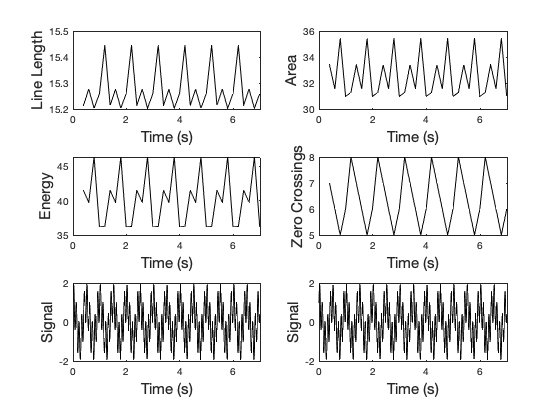
\includegraphics [width=5in]{spatank_hw3_02.png}

  \end{enumerate}
\end{enumerate}
\section{Feature Overlays (17 pts)}
In this section, you will use a line-length feature overlay on a segment of EEG containing a seizure. This data is stored in \texttt{I521\_A0003\_D001}
\begin{enumerate}
 \item What is the length using hours:minutes:seconds:milliseconds of the recording? (Use getDuration) (2 pts)

\begin{lstlisting}
addpath(genpath('ieeg-matlab-1.14.49'))

session_1 = IEEGSession('I521_A0003_D001', 'spatank', 'spa_ieeglogin.bin');
IEEG_signal_duration = session_1.data(1).rawChannels(1).get_tsdetails.getDuration;
IEEG_signal_duration = IEEG_signal_duration/1000; % ms

hours = floor(IEEG_signal_duration/(60 * 60 * 1000))
remainder = rem(IEEG_signal_duration, 60 * 60 * 1000);

minutes = floor(remainder/(60 * 1000))
remainder = rem(remainder, 60 * 1000);

seconds = floor(remainder/1000)
milliseconds = rem(remainder, 1000)
\end{lstlisting}

\color{lightgray} \begin{lstlisting}IEEGSETUP: Adding 'ieeg-matlab.jar' to dynamic classpath
IEEGSETUP: Found log4j on Java classpath.
URL: https://www.ieeg.org/services
Client user: spatank
Client password: ****

hours =

     1


minutes =

    21


seconds =

    20


milliseconds =

   390

\end{lstlisting} \color{black}

 \item How many data points should we discard at the end if we want to clip the recording to the last full second? Do this clipping. (1 pt)

\begin{lstlisting}
remove_duration = milliseconds/1000; % s
sampling_rate = session_1.data.sampleRate;
remove_points = (remove_duration * sampling_rate) + 1

end_time = session_1.data.rawChannels(1).get_tsdetails.getEndTime/1e6; % s
chirp_signal = session_1.data.getvalues(1:ceil(end_time * sampling_rate), 1);

all_seconds = (hours * 60 * 60) + (minutes * 60) + seconds;
dt = 1/sampling_rate;
chirp_time = 0:dt:all_seconds - dt;
chirp_signal = chirp_signal(1:end-remove_points); % clipped to nearest second
\end{lstlisting}

\color{lightgray} \begin{lstlisting}
remove_points =

    79

\end{lstlisting} \color{black}

 \item If we want to overlay a feature trace on the original signal, we have to interpolate that feature (which has been calculated over windows) for each data point of the original signal. One of the simplest methods of doing this is called zero-order interpolation, where we just hold the value constant until we get to the next calculated value. For example, if we had a moving window of 1 second with 1 second displacement, the zero-order interpolated feature vector would have the same value the entire first second, then the same for the entire second second, etc, where each second contains the same number of points as the sampling frequency of the original signal.
 \begin{enumerate}
  \item Using the \texttt{repmat} and \texttt{reshape} functions, create an external function \texttt{zoInterp(x, numInterp} that copies each value of \texttt{x} \texttt{numInterp} times. You can implement this function in one line of code with no loops. Include the code for this function as you did in Question 1.3.a. (2 pts)


  \item Confirm that this function works correctly by expanding the length of the vector \texttt{1:5} by a factor of 5 and plotting with the command
  \begin{lstlisting}
	plot(zoInterp(1:5,5),'-o')
  \end{lstlisting}
  where the \texttt{'-o'} option lets us see the individul points as well as the line that connects them. (2 pts)
 \end{enumerate}

\begin{lstlisting}
figure;
plot(zoInterp(1:5, 5), '-o', 'LineWidth', 1, 'Color', [0, 0, 0])
title('Replication Test', 'FontSize', 15);
\end{lstlisting}


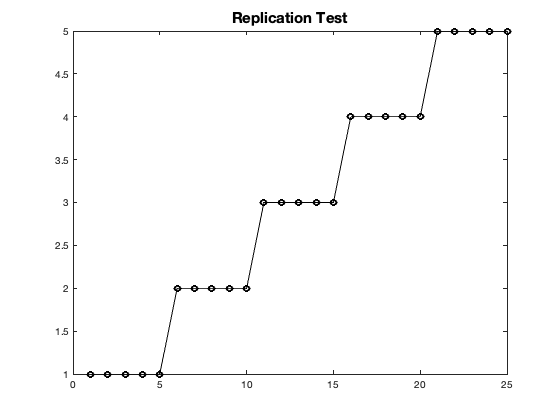
\includegraphics [width=5in]{spatank_hw3_03.png}

 \item Using a 5-second sliding window with 1-second displacement,
 calculate the line length feature over the entire signal. Normalize
 the line-length feature values to have a maximum twice that of the
 original EEG signal maximum. Plot the signal in blue and overlay
 the right-aligned line-length feature in yellow. Note: you will need
 to pad your
 signal in order to get them to line up correctly and be the
 same length. Put the units of your time axis in minutes, and be
 sure to add a legend in a location in the plot that does not cover
 up any signal or feature. (6 pts)

\begin{lstlisting}
winLen = 5; % s
winDisp = 1; % s

LL_chirp = MovingWinFeats(chirp_signal, sampling_rate, winLen, winDisp, LLFn);
LL_chirp_interp = [LL_chirp(1) .* ones(1, (winLen - winDisp) .* sampling_rate), ...
    zoInterp(LL_chirp, winDisp * sampling_rate)];

LL_chirp_norm = (LL_chirp .* 2 .* max(chirp_signal))./max(LL_chirp);

LL_chirp_norm_interp = [LL_chirp_norm(1) .* ones(1, (winLen - winDisp) .* sampling_rate), ...
    zoInterp(LL_chirp_norm, winDisp * sampling_rate)];

figure;
hold on
chirp_time_mins = chirp_time ./ 60;
plot(chirp_time_mins, chirp_signal, 'LineWidth', 2, ...
    'Color', 'b');
plot(chirp_time_mins, LL_chirp_norm_interp, 'LineWidth', 2, ...
    'Color', 'y');
xlim([0, chirp_time_mins(end)])
legend('Signal', 'Normalized Line Length', 'Location', 'NorthWest');
hold off
xlabel('Time (min)', 'FontSize', 15);
title('Normalized Line Length for I521\_A0003\_D001', 'FontSize', 15);
\end{lstlisting}


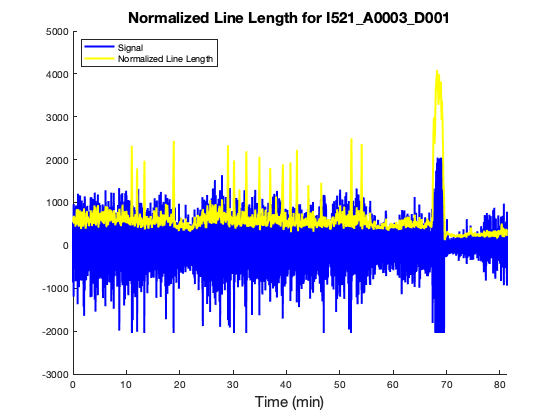
\includegraphics [width=5in]{spatank_hw3_04.png}

 \item What threshold might you use on the raw line-length feature
 vector (not the normalized one used for plotting) in order to
 capture the 17 largest pre-seizure chirps that occur? (1 pt)

\begin{lstlisting}
figure;
plot(chirp_time_mins, LL_chirp_interp, 'LineWidth', 2, ...
    'Color', 'k');
xlabel('Time (min)', 'FontSize', 15);
title('Line Length (I521\_A0003\_D001)', 'FontSize', 15);

threshold = 42000; % for 17 pre-seizure chirps
% threshold = 44000; % for 16 pre-seizure chirps + seizure onset
fprintf('Threshold = %.1f for 17 chirps.\n', threshold);
\end{lstlisting}

\color{lightgray} \begin{lstlisting}Threshold = 42000.0 for 17 chirps.
\end{lstlisting} \color{black}


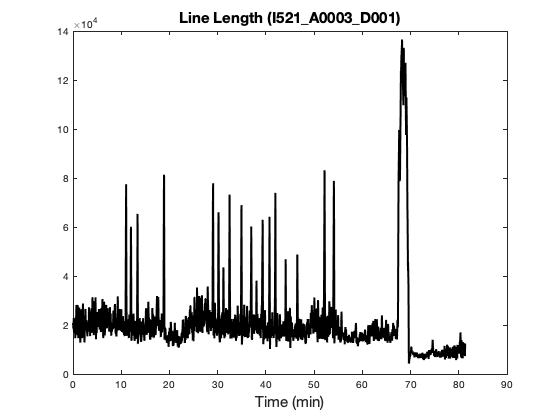
\includegraphics [width=5in]{spatank_hw3_05.png}

 \item Using this threshold value, in another plot draw red vertical lines at the leading point in time where the threshold is crossed. Add these vertical lines on top of the plot you made in Question 2.4. These events should capture the pre-seizure chirps, the seizure onset, and some flickering during the end of the seizure. (3 pts)

\begin{lstlisting}
inds_all = find(LL_chirp_interp >= threshold); % index into signal
inds_val = find(LL_chirp_interp(inds_all - 1) < threshold); % index into index
inds = inds_all(inds_val);

figure;
hold on
chirp_time_mins = chirp_time ./ 60;
plot(chirp_time_mins, chirp_signal, 'LineWidth', 2, ...
    'Color', 'b');
plot(chirp_time_mins, LL_chirp_norm_interp, 'LineWidth', 2, ...
    'Color', 'y');
plot([chirp_time_mins(inds); chirp_time_mins(inds)], ...
    repmat(ylim', 1, size(inds, 2)), '-r', 'LineWidth', 0.75)
xlim([0, chirp_time_mins(end)])
legend('Signal', 'Normalized Line Length', 'Location', 'NorthWest');
hold off
xlabel('Time (min)', 'FontSize', 15);
title('Normalized Line Length (I521\_A0003\_D001)', 'FontSize', 15);
\end{lstlisting}


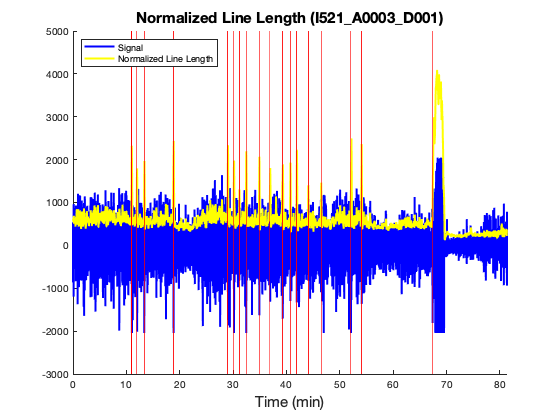
\includegraphics [width=5in]{spatank_hw3_06.png}

\end{enumerate}
\section{Building a Detector (12 pts)}
In this section, you will use the features you defined previously to build a seizure detector. Use the EEG data in the file \texttt{I521\_A0003\_D002} with channels \texttt{multiSz\_1}, and \texttt{multiSz\_2}.
\begin{enumerate}
 \item Plot the signal in \texttt{multiSz\_1} and draw vertical red lines at the times when you think the two seizures begin. (You should be able to do this without the need of any features.) (2 pts)

\begin{lstlisting}
session_2 = IEEGSession('I521_A0003_D002', 'spatank', 'spa_ieeglogin.bin');
sampling_rate = session_2.data.sampleRate;

end_time = session_2.data.rawChannels(1).get_tsdetails.getEndTime/1e6; % s
multiSz_1 = session_2.data.getvalues(1:ceil(end_time * sampling_rate), 1);

dt = 1/sampling_rate;
time_multiSz_1 = 0:dt:end_time;

seizure_inds = [755, 9382];

figure;
hold on
plot(time_multiSz_1, multiSz_1, 'LineWidth', 1, 'Color', [0, 0, 0])
plot([seizure_inds; seizure_inds], ...
    repmat(ylim', 1, size(seizure_inds, 2)), '-r', 'LineWidth', 2)
hold off
xlabel('Time (s)', 'FontSize', 15);
ylabel('Signal', 'FontSize', 15);
title('Channel 1 (I521\_A0003\_D002)', 'FontSize', 15);
\end{lstlisting}

\color{lightgray} \begin{lstlisting}IEEGSETUP: Adding 'ieeg-matlab.jar' to dynamic classpath
Warning: Objects of edu/upenn/cis/db/mefview/services/TimeSeriesDetails class
exist - not clearing java 
Warning: Objects of edu/upenn/cis/db/mefview/services/TimeSeriesInterface class
exist - not clearing java 
IEEGSETUP: Found log4j on Java classpath.
URL: https://www.ieeg.org/services
Client user: spatank
Client password: ****
\end{lstlisting} \color{black}


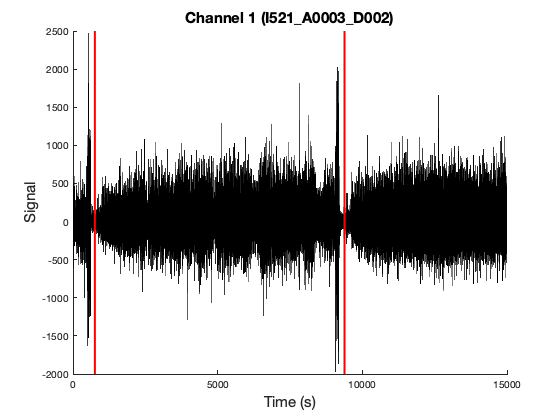
\includegraphics [width=5in]{spatank_hw3_07.png}

 \item Produce feature overlay plots similar to that of Question 2.4 for each of the four features you have implemented along with the red vertical lines at each seizure. Use the same 4-second sliding window with 1 second displacement. (4 pts)

\begin{lstlisting}
winLen = 0.4; % s
winDisp = 0.1; % s

multiSz_1_LL = MovingWinFeats(multiSz_1, sampling_rate, winLen, winDisp, LLFn);
multiSz_1_area = MovingWinFeats(multiSz_1, sampling_rate, winLen, winDisp, areaFn);
multiSz_1_energy = MovingWinFeats(multiSz_1, sampling_rate, winLen, winDisp, energyFn);
multiSz_1_ZC = MovingWinFeats(multiSz_1, sampling_rate, winLen, winDisp, ZCFn);

multiSz_1_LL_interp = [multiSz_1_LL(1) .* ...
    ones(1, round((winLen - winDisp) .* sampling_rate)), ...
    zoInterp(multiSz_1_LL, winDisp * sampling_rate)];
multiSz_1_area_interp = [multiSz_1_area(1) .* ...
    ones(1, round((winLen - winDisp) .* sampling_rate)), ...
    zoInterp(multiSz_1_area, winDisp * sampling_rate)];
multiSz_1_energy_interp = [multiSz_1_energy(1) .* ...
    ones(1, round((winLen - winDisp) .* sampling_rate)), ...
    zoInterp(multiSz_1_energy, winDisp * sampling_rate)];
multiSz_1_ZC_interp = [multiSz_1_ZC(1) .* ...
    ones(1, round((winLen - winDisp) .* sampling_rate)), ...
    zoInterp(multiSz_1_ZC, winDisp * sampling_rate)];

multiSz_1_LL_interp = (multiSz_1_LL_interp .* 2 .* max(multiSz_1))./max(multiSz_1_LL_interp);
multiSz_1_area_interp = (multiSz_1_area_interp .* 2 .* max(multiSz_1))./max(multiSz_1_area_interp);
multiSz_1_energy_interp = (multiSz_1_energy_interp .* 2 .* max(multiSz_1))./max(multiSz_1_energy_interp);
multiSz_1_ZC_interp = (multiSz_1_ZC_interp .* 2 .* max(multiSz_1))./max(multiSz_1_ZC_interp);

figure;
hold on
plot(time_multiSz_1, multiSz_1, 'LineWidth', 2, 'Color', 'b')
plot(time_multiSz_1, multiSz_1_LL_interp, 'LineWidth', 2, 'Color', 'r')
plot([seizure_inds; seizure_inds], ...
    repmat(ylim', 1, size(seizure_inds, 2)), '-r', 'LineWidth', 2)
hold off
xlim([0, end_time])
legend('Raw Signal', 'Normalized Line Length', 'Location', 'NorthEast')
title('Line Length (I521\_A0003\_D002 Ch. 1)', 'FontSize', 15);
xlabel('Time (s)', 'FontSize', 15);
ylabel('Line Length', 'FontSize', 15);

figure;
hold on
plot(time_multiSz_1, multiSz_1, 'LineWidth', 2, 'Color', 'b')
plot(time_multiSz_1, multiSz_1_area_interp, 'LineWidth', 2, 'Color', 'r')
plot([seizure_inds; seizure_inds], ...
    repmat(ylim', 1, size(seizure_inds, 2)), '-r', 'LineWidth', 2)
hold off
xlim([0, end_time])
legend('Raw Signal', 'Normalized Area', 'Location', 'NorthEast')
title('Area (I521\_A0003\_D002 Ch. 1)', 'FontSize', 15);
xlabel('Time (s)', 'FontSize', 15);
ylabel('Area', 'FontSize', 15);

figure;
hold on
plot(time_multiSz_1, multiSz_1, 'LineWidth', 2, 'Color', 'b')
plot(time_multiSz_1, multiSz_1_energy_interp, 'LineWidth', 2, 'Color', 'r')
plot([seizure_inds; seizure_inds], ...
    repmat(ylim', 1, size(seizure_inds, 2)), '-r', 'LineWidth', 2)
hold off
xlim([0, end_time])
legend('Raw Signal', 'Normalized Energy', 'Location', 'NorthEast')
title('Energy (I521\_A0003\_D002 Ch. 1)', 'FontSize', 15);
xlabel('Time (s)', 'FontSize', 15);
ylabel('Energy', 'FontSize', 15);

figure;
hold on
plot(time_multiSz_1, multiSz_1, 'LineWidth', 2, 'Color', 'b')
plot(time_multiSz_1, multiSz_1_ZC_interp, 'LineWidth', 2, 'Color', 'r')
plot([seizure_inds; seizure_inds], ...
    repmat(ylim', 1, size(seizure_inds, 2)), '-r', 'LineWidth', 2)
hold off
xlim([0, end_time])
legend('Raw Signal', 'Normalized Zero Crossings', 'Location', 'SouthEast')
title('Zero Crossings (I521\_A0003\_D002 Ch. 1)', 'FontSize', 15);
xlabel('Time (s)', 'FontSize', 15);
ylabel('Zero Crossings', 'FontSize', 15);
\end{lstlisting}


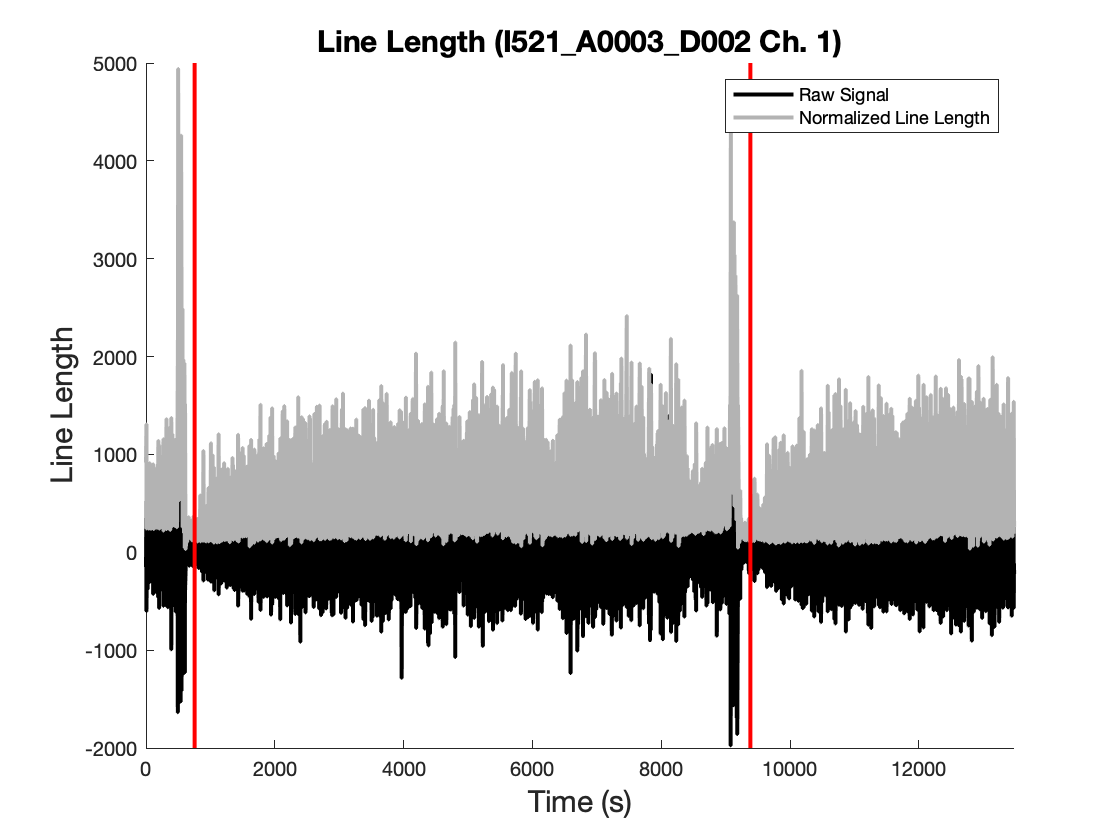
\includegraphics [width=5in]{spatank_hw3_08.png}


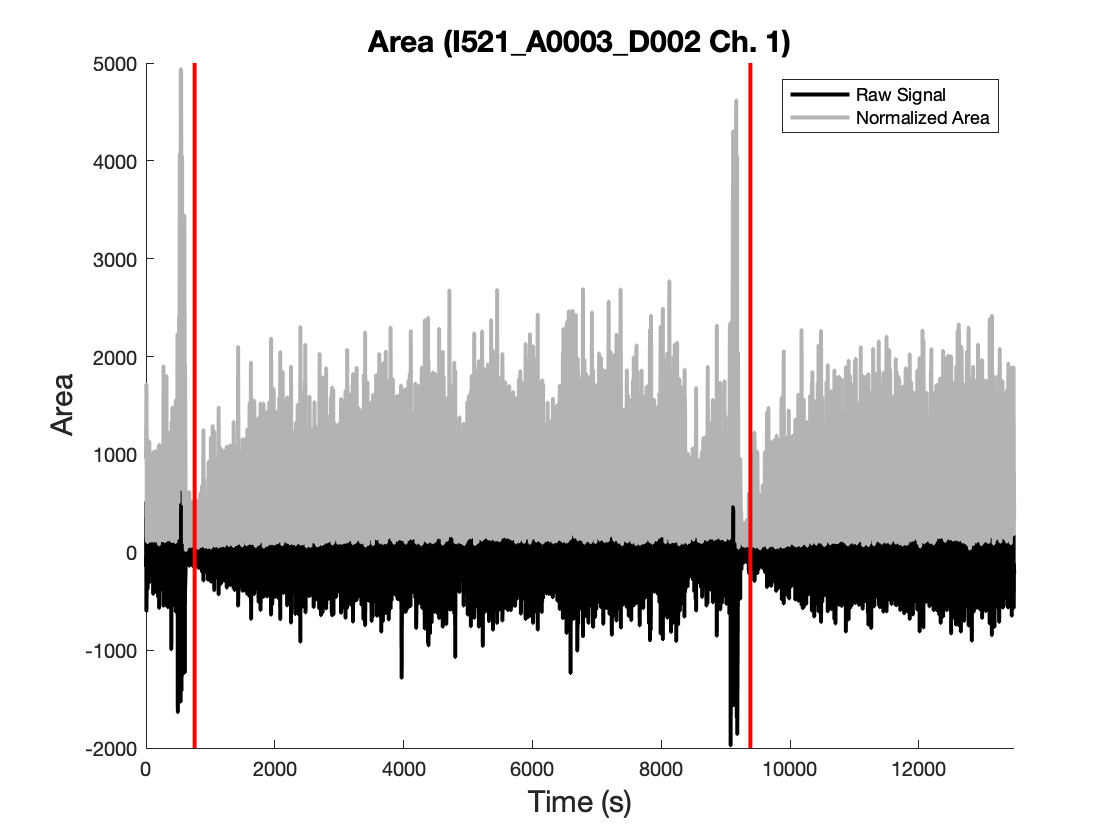
\includegraphics [width=5in]{spatank_hw3_09.png}


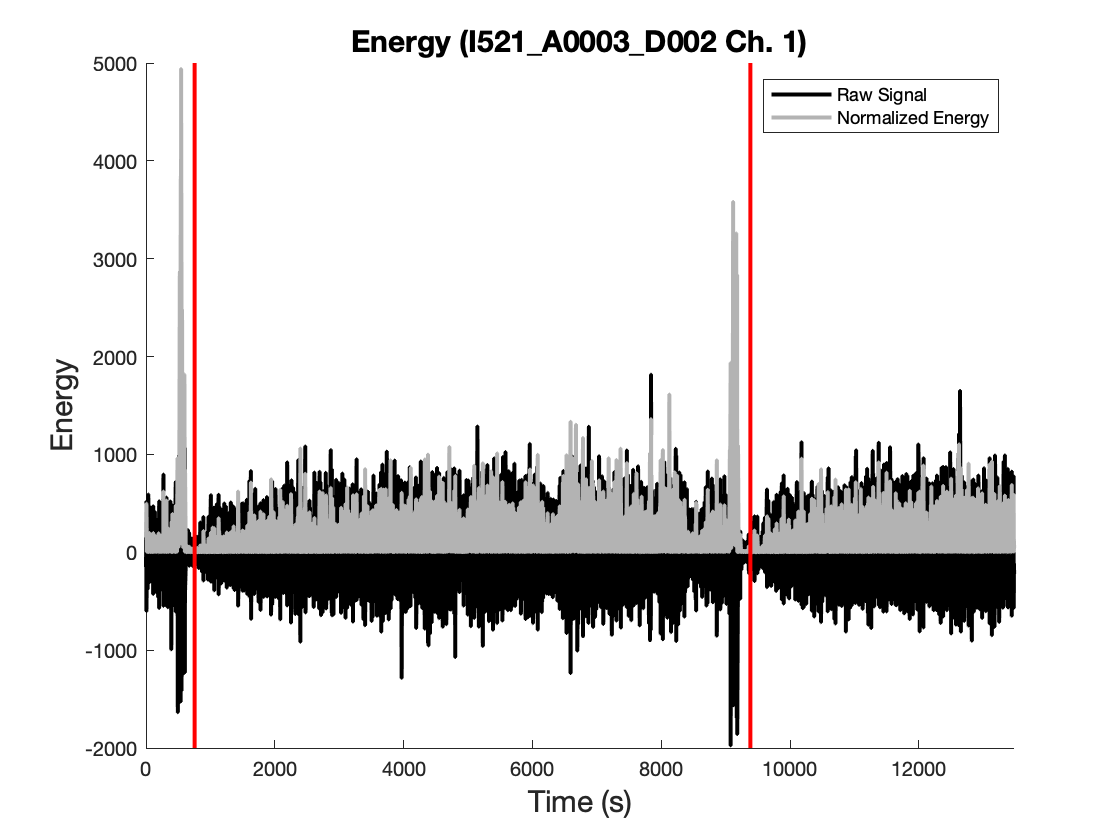
\includegraphics [width=5in]{spatank_hw3_10.png}


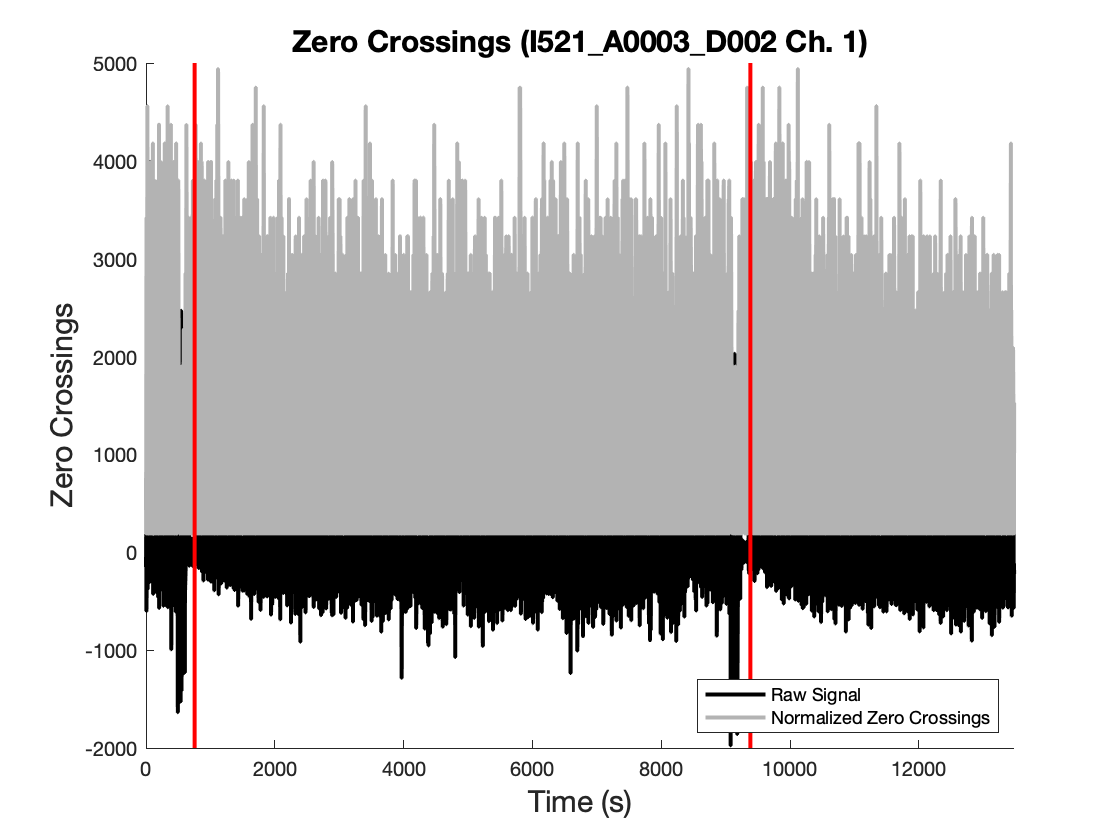
\includegraphics [width=5in]{spatank_hw3_11.png}

 \item
  \begin{enumerate}
   \item Based on your plots in the previous question, which of the
   four features seems to give the largest signal (relative to the
   background) for when a seizure occurs? Explain why you think this feature is the best. (3 pts)

\begin{lstlisting}
% Energy seems to give the largest signal relative to the background before
% a seizure. There are significant pre-seizure spikes in line length, area,
% and energy. However, the difference in values between the spike and the
% mean for line length and area is much smaller compared to the same
% difference for energy. Zero crossings on the other hand are much noisier
% compared to the other three features.
\end{lstlisting}

   \item What threshold would you use to determine if a seizure is occurring? (1 pt)

\begin{lstlisting}
% Normalized energy exceeding 3000 is a strong indicator of an imminent seizure.
threshold = 3000; % energy threshold for seizure
\end{lstlisting}

  \end{enumerate}


 \item The signal in \texttt{multiSz\_2} contains another seizure (whose location should again be fairly obvious). Plot the data along with the feature and threshold (horizontal black line, with correct normalization for the signal in \texttt{data2}) you determined in the previous question. (2 pts)

\begin{lstlisting}
signal_duration = session_2.data(1).rawChannels(2).get_tsdetails.getDuration;
signal_duration = signal_duration/1e6; % s
sampling_rate = session_2.data.sampleRate;

end_time = session_2.data.rawChannels(2).get_tsdetails.getEndTime/1e6; % s
multiSz_2 = session_2.data.getvalues(1:ceil(end_time * sampling_rate), 2);

dt = 1/sampling_rate;
time_multiSz_2 = 0:dt:end_time;

winLen = 0.4; % s
winDisp = 0.1; % s

multiSz_2_energy = MovingWinFeats(multiSz_2, sampling_rate, winLen, winDisp, energyFn);
multiSz_2_energy_interp = [multiSz_2_energy(1) .* ...
    ones(1, round((winLen - winDisp) .* sampling_rate)), ...
    zoInterp(multiSz_2_energy, winDisp * sampling_rate)];
multiSz_2_energy_interp_norm = (multiSz_2_energy_interp .* 2 .* max(multiSz_2))./max(multiSz_2_energy_interp);

figure;
hold on
plot(time_multiSz_2, multiSz_2, 'LineWidth', 1, 'Color', 'b')
plot(time_multiSz_2, multiSz_2_energy_interp_norm, 'LineWidth', 1, ...
    'Color', 'r')
line([0, time_multiSz_2(end)], [threshold, threshold], 'LineWidth', 1, ...
    'Color', [0, 0, 0])
hold off
legend('Signal', 'Normalized Energy', 'Threshold', 'Location', 'NorthEast');
xlabel('Time (s)', 'FontSize', 15);
title('Channel 2 (I521\_A0003\_D002)', 'FontSize', 15);
\end{lstlisting}


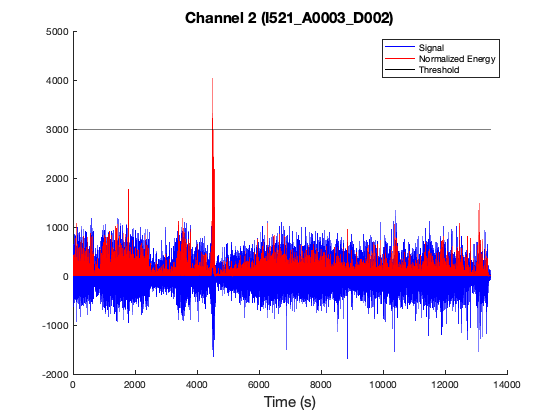
\includegraphics [width=5in]{spatank_hw3_12.png}

\end{enumerate}




\end{document}
    
